%----------------------------------------------------------------
%
%  File    :  thesis.tex
%
%  Authors :  Keith Andrews, IICM, TU Graz, Austria
%             Manuel Koschuch, FH Campus Wien, Austria
%			  Sebastian Ukleja, FH Campus Wien, Austria
% 
%  Created :  22 Feb 96
% 
%  Changed :  14 Oct 2020
%
%  For suggestions and remarks write to: sebastian.ukleja@fh-campuswien.ac.at
% 
%----------------------------------------------------------------

% --- Setup for the document ------------------------------------

%Class for a book like style:
\documentclass[11pt,a4paper,oneside]{scrbook}
%For a more paper like style use this class instead:
%\documentclass[11pt,a4paper,oneside]{thesis}

%input encoding for windows in utf-8 needed for Ä,Ö,Ü etc..:
\usepackage[utf8]{inputenc}
%input encoding for linux:
%\usepackage[latin1]{inputenc}
%input encoding for mac:
%\usepackage[applemac]{inputenc}

\usepackage[english]{babel}
% for german use this line instead:
%\usepackage[ngerman]{babel}

%needed for font encoding
\usepackage[T1]{fontenc}

% want Arial? uncomment next two lines...
%\usepackage{uarial}
%\renewcommand{\familydefault}{\sfdefault}

%some formatting packages
\usepackage[bf,sf]{subfigure}
\renewcommand{\subfigtopskip}{0mm}
\renewcommand{\subfigcapmargin}{0mm}

%For better font resolution in pdf files
\usepackage{lmodern}

\usepackage{url}

%\usepackage{latexsym}

\usepackage{geometry} % define pagesize in more detail


\usepackage{colortbl} % define colored backgrounds for tables

\usepackage{courier} %for listings
\usepackage{listings} % nicer code formatting
\lstset{basicstyle=\ttfamily,breaklines=true}

\usepackage{graphicx}
  \pdfcompresslevel=9
  \pdfpageheight=297mm
  \pdfpagewidth=210mm
  \usepackage[         % hyperref should be last package loaded
    pdftex, 		   % needed for pdf compiling, DO NOT compile with LaTeX
    bookmarks,
    bookmarksnumbered,
    linktocpage,
    pagebackref,
    pdfview={Fit},
    pdfstartview={Fit},
    pdfpagemode=UseOutlines,                 % open bookmarks in Acrobat
  ]{hyperref}
\DeclareGraphicsExtensions{.pdf,.jpg,.png}
\usepackage{bookmark}

\usepackage[title]{appendix}

%paper format
\geometry{a4paper,left=30mm,right=25mm, top=30mm, bottom=30mm}

% --- Settings for header and footer ---------------------------------
\usepackage{scrlayer-scrpage}
\clearscrheadfoot
\pagestyle{scrheadings}
\automark{chapter}

%Left header shows chapter and chapter name, will not display on first chapter page use \ihead*{\leftmark} to show on every page
\ihead{\leftmark} 	
%\ohead*{\rightmark}	%optional right header
\ifoot*{Ursula Rauch}		%left footer shows student name
\ofoot*{\thepage}		%right footer shows pagination
%---------------------------------------------------------------------

%--- additional packages necessary for table in results --------------
\usepackage[xcdraw]{xcolor}
\usepackage{lscape}
%-------------------------------------------------------------------- 

\usepackage{xcolor}

%New colors defined below
\definecolor{codegreen}{rgb}{0,0.6,0}
\definecolor{codegray}{rgb}{0.5,0.5,0.5}
\definecolor{codepurple}{rgb}{0.58,0,0.82}
\definecolor{backcolour}{rgb}{0.95,0.95,0.92}

%Code listing style named "mystyle"
\lstdefinestyle{mystyle}{
  backgroundcolor=\color{backcolour}, commentstyle=\color{codegreen},
  keywordstyle=\color{magenta},
  numberstyle=\tiny\color{codegray},
  stringstyle=\color{codepurple},
  basicstyle=\ttfamily\footnotesize,
  breakatwhitespace=false,
  breaklines=true,
  captionpos=b,
  keepspaces=true,
  numbers=left,
  numbersep=5pt,
  showspaces=false,
  showstringspaces=false,
  showtabs=false,
  tabsize=2
}
\lstset{style=mystyle}
%----------------------------

%Start of your document beginning with title page
\begin{document}


% --- Main Title Page ------------------------------------------------
\begin{titlepage}
\frontmatter

\begin{picture}(50,50)
\put(-70,40){\hbox{
\includegraphics{images/logo.png}}}
\end{picture}

\vspace*{-5.8cm}

\begin{center}

\vspace{6.2cm}

\hspace*{-1.0cm} {\LARGE \textbf{The positioning of the OAuth2 client in a Microservice-based Architecture\\}}
\vspace{0.2cm}
\hspace*{-1.0cm} A comparison between the implementation of the OAuth2 client in the Gateway and in the frontend\\

\vspace{2.0cm}

\hspace*{-1.0cm} { \textbf{Bachelor Thesis\\}}

\vspace{0.65cm}

\hspace*{-1.0cm} Submitted in partial fulfillment of the requirements for the degree of \\

\vspace{0.65cm}

\hspace*{-1.0cm} \textbf{Bachelor of Science in Engineering\\}

\vspace{0.65cm}

\hspace*{-1.0cm} to the University of Applied Sciences FH Campus Wien \\
\vspace{0.2cm}
\hspace*{-1.0cm} Bachelor Degree Program: Computer Science and Digital Communications \\

\vspace{1.6cm}

\hspace*{-1.0cm} \textbf{Author:} \\
\vspace{0.2cm}
\hspace*{-1.0cm} Ursula Rauch \\

\vspace{0.7cm}

\hspace*{-1.0cm} \textbf{Student identification number:}\\
\vspace{0.2cm}
\hspace*{-1.0cm} 00514397 \\

\vspace{0.7cm}

\hspace*{-1.0cm} \textbf{Supervisor:} \\
\vspace{0.2cm}
\hspace*{-1.0cm} Leon Freudenthaler, BSc MSc \\

\vspace{0.7cm}

% Reviewer if needed
%\hspace*{-1.0cm} \textbf{Reviewer: (optional)} \\
%\vspace{0.2cm}
%\hspace*{-1.0cm} Title first name surname \\


\vspace{1.0cm}

\hspace*{-1.0cm} \textbf{Date:} \\
\vspace{0.2cm}
\hspace*{-1.0cm}!!!FEHLT NOCH!!! \\

\end{center}
\end{titlepage}

\newpage

\vspace*{16cm}
\setcounter{page}{1}

% --- Declaration of authorship ------------------------------------------
\hspace*{-0.7cm} \underline{Declaration of authorship:}\\\\
I declare that this Bachelor Thesis has been written by myself. I have not used any other than the listed sources, nor have I received any unauthorized help.\\\\
I hereby certify that I have not submitted this Bachelor Thesis in any form (to a reviewer for assessment) either in Austria or abroad.\\\\
Furthermore, I assure that the (printed and electronic) copies I have submitted are identical.
\\\\\\
Date: 15.01.2023 \hspace{6cm} Signature:\\

% --- English Abstract ----------------------------------------------------
\cleardoublepage
\chapter*{Abstract}
This thesis investigates different implementations of Authorization and Authentication with OpenID Connect (OIDC) and OAuth 2.0 (OAuth2) in a microservice architecture (MSA) environment...
% --- German Abstract ----------------------------------------------------
\cleardoublepage
\chapter*{Kurzfassung}
Diese Arbeit untersucht unterschiedliche Implementierungen von OpenID Connect (OIDC) bzw. OAuth 2.0 (OAuth2) im Kontext von \linebreak Microservice-Architekturen (MSA) ...

% --- Abbrevations ----------------------------------------------------
\chapter*{List of Abbreviations}
\vspace{0.65cm}

\begin{table*}[htbp]
		\begin{tabular}{ll}
			!!!ALT! NICHT gebrauchte raushaun!
			BCP & Best Current Practice \\
			CRUD & Create Read Update Delete \\
			ECDSA & Elliptic Curve Digital Signature Algorithm \\
			ES256 & ECDSA SHA-256 \\
			HMAC & Hash-based Message Authentication Code \\
			HS256 & HMAC SHA-256 \\
			IANA & Internet Assigned Numbers Authority \\
			IETF & Internet Engineering Task Force \\
			JOSE & JavaScript Object Signing and Encryption \\
			JSON & JavaScript Object Notation \\
			JWE & JSON Web Encryption \\			
			JWS & JSON Web Signature \\
			JWT & JSON Web Token \\
			MSA & Microservice Architecture \\
			OIDC & OpenID Connect \\
			RFC & Request for Comments \\
			POC & Proof of Concept \\
			RSA & Rivest-Shamir-Adelman \\
			%SAML & Secturity Asertion Markup Language \\
			SHA & Secure Hash Algorithm \\
			SSO & Single Sign-on \\
			XACML & Extensible Access Control Markup Language \\
		\end{tabular}
\end{table*}

% --- Key terms ----------------------------------------------------
\newpage
\chapter*{Key Terms}
\vspace{0.65cm}

\begin{itemize}
	\setlength{\itemsep}{0pt}
	\item[] Authentication
	\item[] Authorization
	\item[] BFF
	\item[] Gateway
	\item[] JWT
	\item[] Microservice Architecture
	\item[] OAuth 2
	\item[] OpenID Connect
\end{itemize}

% --- Table of contents autogenerated ------------------------------------
\newpage
\tableofcontents
\thispagestyle{empty}

% --- Begin of Thesis ----------------------------------------------------
\mainmatter
 \chapter{Introduction}
\label{chap:intro}

!!! Einleitung allgemein, Forschungsfragen:

Die Rolle des Gateways für Authentifizierung und Autorisierung mit Oauth2 und OpenID
Connect in Microservice-basierten Architekturen. Das Gateway kann sowohl als OAuth2-Client,
als auch als Resource Server implementiert werden. Im ersten Fall muss das Gateway als Client einen Access Token vom Authorization Server beantragen und diesen an den Resource
Server, also einen dahinter liegenden Service weiterschicken. Wenn das Gateway selbst als
Resource Server implementiert ist, muss das Frontend als Client fungieren und den Access Token beschaffen.
//
Forschungsfrage:
Wie lassen sich beide Patterns mit Spring Boot implementieren? Welche Unterschiede gibt es
zwischen den Varianten, z.B. in den Bereichen Performance, Sicherheit, Komplexität?

\section{Related Work}
\label{sec:relwork}


 \section{Microservice-based vs Monolithic Architecture}
\label{sec:msa-mon}

%!!! sicherheitshalber aus der BA1 zitieren!
\begin{figure}[htbp]
	\centering
		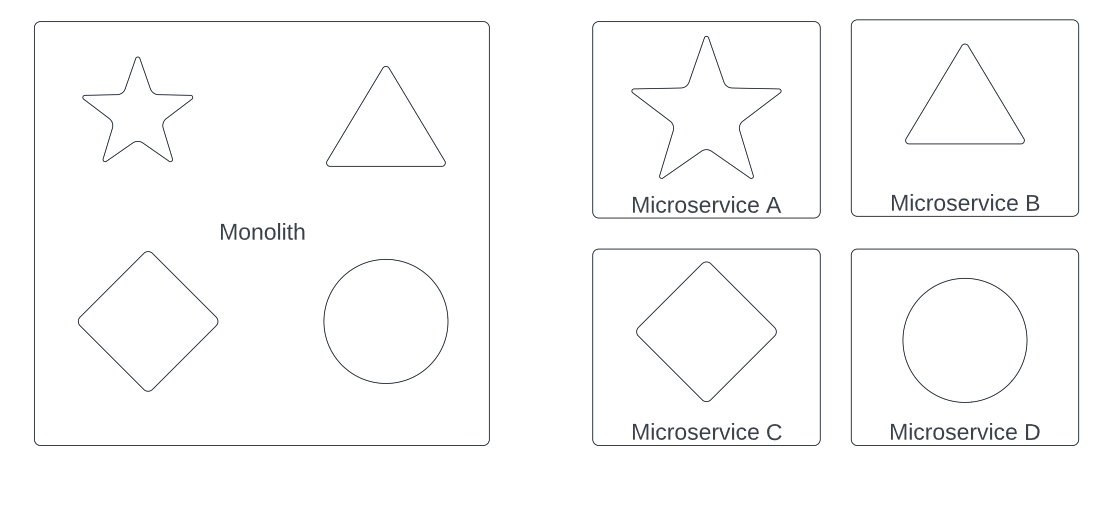
\includegraphics[width=\textwidth]{images/microservices-monolith.png}
	\caption{A very abstract illustration of a monolith and micoservices according to \cite{lewis_microservices_2014}}
	\label{fig:msa}
\end{figure}


\section{MSA Security Challenges}
\label{sec:security}
!!! weglassen?

\section{Authentication and Authorization}
\label{sec:authx}

!!! ALT - Neu formulieren
As we have seen in the previous sections, when talking about security in microservices, both, authentication and authorization are considered to be among the most important topics. In this section, a clarification is given how the two concepts differ and what their role is in the context of MSA. % and they are also discussed the most in academic literature (wie isses mit grey lit.?) (Billawa et al.).\\

Authentication and authorization, although they sound very similar, are two distinctive concepts and it is important to understand the difference between the two.
To put it very shortly, authentication is about identity and authorization is about permissions. When someone authenticates, they usually provide a proof of the fact that what they say who they are is true. Identity can be proven with something they know (e.g., a secret password), something they have (like a phone number, to which a code can be sent), or something they are (like biometric data), or a combination of those (e.g. in two-factor authentication where a user gives their username and password, but the authentication is only complete when they also give a code that was sent to their phone number or e-mail address). Not only a person can prove their identity. A system can authenticate as well, for example with a secret or certificate or both. Authorization on the other hand deals with the question what a person or entity is allowed to do, for example where they can enter. Because this usually depends on who they are, in order to determine which permissions someone or something has, authentication is necessary first. Siriwardena \cite[p.~133]{siriwardena_advanced_2020} gives a visa control at a border as example: A person who wants to cross the border has to authenticate - their picture and/or fingerprint might be validated as truly belonging to that person, perhaps also by comparing to a database. This is authentication. Knowing who that person is does not get this person across the border, unless they have a visa. The visa has to be valid and not expired and can contain further details about what you are allowed to do in that country \cite[p.~133]{siriwardena_advanced_2020}.
%siehe auhc chocolate vs. fudge oauth.net/articles/authentication Justin Richer)\\

%vergleich mit monolithic a. -> Nic Jackson auch noch angeben? wegen den tokens warats
Now, what is special about authentication and authorization in a MSA? In a monolithic architecture, when a user wants to access a resource, they authenticate with the system and might get back a session token, which can be sent with every subsequent request to the system. The token can then be validated inside the system, and it will know if this user has the necessary permission for the requested transaction. The same process becomes way more complex in MSA. While a monolithic application only has few entry points, a MSA has at least as many entry points as deployed services and each of them should be protected \cite{jackson_microservice_2019}, \cite{dragoni_microservices_2017}. When a requested resource or service does not sit inside the same system as the service where the user has authenticated themselves, the first service does not know if it can trust whoever made this request without either making another request to the server responsible for dealing with authentication and permissions, or having a way to validate the token locally, without further communication, which might not always be possible. This results in a higher number of requests between services and therefore in potentially decreased performance of the MSA.% \cite{siriwardena_microservices_2020}.\\

To make everything worse, not only access by external end-users has to be managed, but also communication between services. Although the MSA principle demands loosely coupled microservices, it is sometimes inevitable that one service has to talk to another service in order to fulfil its job. But a service should not be reachable by any other microservices in the system, only by those who have a good reason to do so \cite{yarygina_overcoming_2018}. When a service talks to another service on behalf of a user, the user information (authentication and authorization) can be passed on down the line, so each microservice knows who they are working for. This is called principal propagation \cite{yarygina_overcoming_2018}.\\

%third-party access...

%oauth2+oidc hier schon ankündigen?



%\subsection{The API Gateway}
%\label{sec:UnterUnterkapitel22}
%Kommt wahrscheinlich raus, sonst hier anmerken, das das wichtig ist, aber in dieser Arbeit nicht weiter behandelt wird.\\

%While there exist different approaches to the implementation of API Gateways in MSA \cite{floren_implementation_2021}, authors seem to generally agree about the need of at least one API Gateway that stands between the client or end user and the backend microservices.!!!da noch wen zitieren? The beforementioned increased attack surface of an MSA can be reduced dramatically by creating a choke point for all requests  
%\end{comment}

\section{Authentication Patterns}
\label{sec:auth-patterns}

!!! Backend for Frontend vs. Frontend als Client + Diagramme. Wireshark eher erst unter implementation?

\section{OAuth2}
\label{sec:oauth2}

Neu: redirect-uri! Wird beim gateway erwähnt!

% fehlt: OAuth2 beliebt in microservices according to literature, academic + grey! (billawa et al., pereira-vale...)
% genauer drauf eingehen, warum oauth2 für microservices???
% artikel von eran hammer (oauth 2.0 and the road to hell) dazu, um zu illustrieren, wie mühsam es ist + aaron parecki, der sich für das labyrinth entschuldigt (how to hack oauth) -> und trotzdem isses so beliebt.
%ref für industy standard? nate barbettini - redet aber nicht über ms spezifisch
OAuth 2.0, also often referred to as OAuth2, is an open protocol for delegated authorization, defined by the Internet Engineering Task Force (IETF) in the Request for Comments (RFC) 6749 \cite{hardt_oauth_2012} and RFC 6750 \cite{jones_oauth_2012}. Authors of grey and academic literature seem to agree that OAuth2 is the standard for authorization in MSA environment (see chapter \ref{chap:relwork}). OAuth2 was developed to allow a third-party client to access a certain (protected) resource on behalf of the owner of this resource \cite{hardt_oauth_2012}. In a MSA environment, where different services and possibly an API Gateway have to communicate with each other on behalf of a user or of another service, this concept of third-party access makes OAuth2 a feasible solution. The access to a resource happens by means of a so-called \textit{access token}, which is issued to the client from an authorization server and which allows the client, now in possession of this token, to access the protected resource. The token now has to be sent with every request to the server holding that resource.
This chapter gives insight into some of the mechanisms and specifications of the OAuth 2.0 protocol. However, this thesis can not cover all the details of OAuth2 and some concepts have to be described in a simplified manner.

\subsection{OAuth2 Roles}
\label{sec:oauthroles}
% eigener abschnitt über implicit und password grant, warum nicht mehr verwenden???
There are four important roles in the OAuth2 authorization flow \cite{hardt_oauth_2012}:
\begin{itemize}
\item  The \textit{resource owner} is the person or entity that owns a protected resource. The resource owner can grant access to this resource to a third party.
\item The \textit{resource server} is the server where the resource in question lives. It responds to requests containing the access token.
\item The \textit{client} is any application (e.g. a web application or a mobile application) requesting the resource. It is not specified where this application is executed. The client can also act on its own behalf when it is the resource owner at the same time. %public vs. confidential clients steht schon weiter unten, kann aber auch hier noch eingebaut werden.
\item The \textit{authorization server} is the server responsible for authentication of the resource owner, obtaining authorization and issuing access tokens to the client.
\end{itemize}
An example scenario to illustrate these roles would be that a user (the resource owner) has a Facebook account and wants another application (the client) to access data (the protected resource) in their account, maybe because the app has promised to analyze the user's personality based on their timeline posts \cite{jackson_microservice_2019}.\\


\subsection{The OAuth2 Authorization Flow}
\label{sec:oauthflow}

\begin{figure}[htbp]
	\centering
		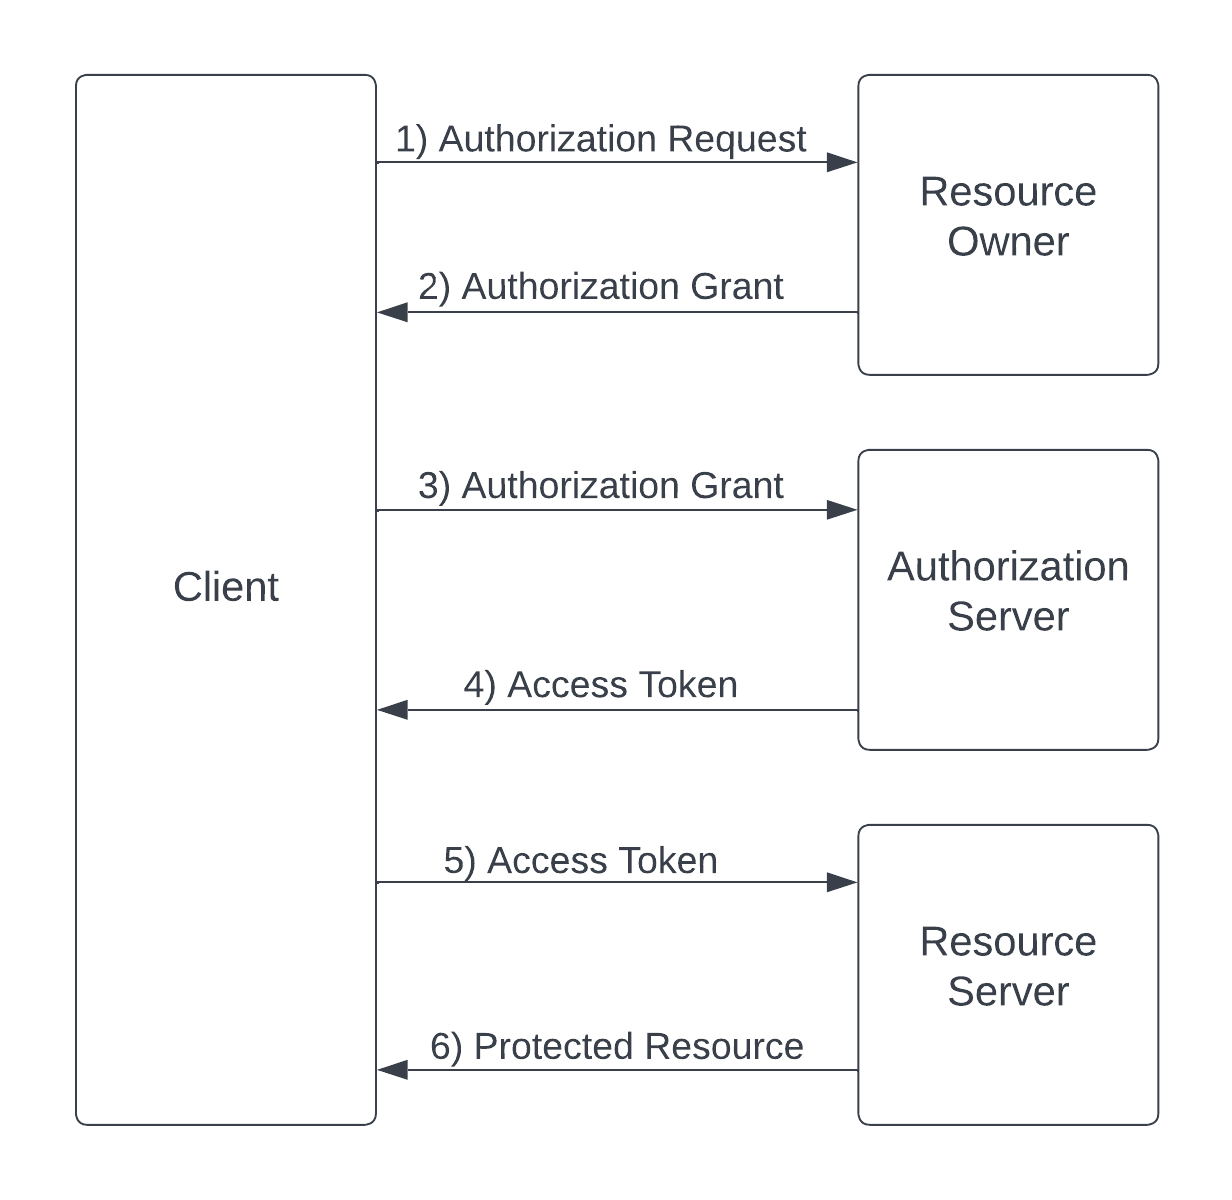
\includegraphics{images/oauth2-flow}
	\caption{Abstraction of the OAuth2 flow after \cite[fig.~1]{hardt_oauth_2012}}
	\label{fig:oauth2flow}
\end{figure}

The simple and most dangerous way for the client to access the user's Facebook data from the example above would be that the user passes their username and password to the client, which can then comfortably log in to the user's Facebook account and do with it whatever it wants to do \cite[p.~81]{siriwardena_advanced_2020}. Obviously, this would lead to many problems if the client, now in possession of the user's credentials, is not trustworthy. OAuth2 solves this problem by enabling the user to grant the client access to their data without letting it see their username and password. This is done by delegating the authorization process to the authorization server. Once the user is authenticated with the authorization server and has given permission to the application to access data from their account, the application will receive the access token and can present this token to the server in exchange for the data they want. The basic steps of the OAuth2 flow are as follows \cite{hardt_oauth_2012} (see also figure \ref{fig:oauth2flow}):%auch auf zeichnung verweisen, sobald die da ist \\
\begin{enumerate}
\item An authorization request is made by the client to the resource owner (preferably via the authorization server)
\item An authorization grant is issued (again preferably via the authorization server) to the client.
\item The client requests an access token from the authorization server by presenting the authorization grant.
\item The access token is issued to the client (after authenticating the client and validating the request).
\item The client presents the access token to the resource server and requests the protected resource.
\item The access token is validated by the resource server (locally or by calling the authorization server) and, if successful, responds with the requested resource. 
\end{enumerate}

In reality the authorization grant, which represents the authorization by the resource owner for the client to access a resource, can come in different shapes. 

\subsection{The OAuth2 Authorization Grant Types}
\label{sec:oauthgrants}
The exact flow in which the client can receive the access token can differ, depending on the \textit{grant type}. The original specification defines four different grant types, but it is also possible to define additional grant types \cite{hardt_oauth_2012}. However, not all of those original grant types are still recommended for implementation according to the OAuth 2.0 Security Best Current Practice (BCP) IETF Internet Draft \cite{lodderstedt_oauth_2022}. %evt. auch noch oauth.net und oauth.com anschaun oder siri
\begin{itemize}
\item With the \textit{authorization code grant}, the authorization server responds to the authorization request (after authenticating the resource owner and obtaining authorization) not with the access token, but with a code, which the resource owner's user-agent (e.g. web-browser) will pass on to the client at the redirection URI \cite{hardt_oauth_2012}. The client can then exchange this code for an access token directly with the authorization server, without exposing the token to the resource owner or potentially anyone else. It is also possible for the authorization server to authenticate the client \cite{hardt_oauth_2012}.
\item The \textit{client credentials} grant: The client receives an access token after authenticating itself to the authorization server with its client credentials (a password or public/private key) \cite{hardt_oauth_2012}.  %With this grant type, no refresh token is issued alongside the access token \cite{siriwardena_advanced_2020}.%??? bessere quelle? nicht in RFC6749 gefunden
\end{itemize}

Legacy grant types \cite{parecki_oauth_granttypes}:
\begin{itemize}
\item The \textit{implicit grant} is similar to the authorization code grant, but here the access token is sent to the client directly instead of sending a code first and the authorization server does not authenticate the client \cite{hardt_oauth_2012}.
\item With the \textit{resource owner password grant}, \texttt{password grant} for short, the resource owner's credentials are directly exchanged for an access token \cite{hardt_oauth_2012}.
\end{itemize}

Other grant types are the \textit{device code} grant, which is an extension \cite{denniss_oauth_2019}, and sometimes also the \textit{refresh token} \cite{hardt_oauth_2012} is called a grant type \cite{parecki_oauth_nodate}, \cite[p.~372]{siriwardena_microservices_2020}, although it is not considered as such in the original OAuth2 specification \cite{hardt_oauth_2012}.

The choice of the grant type depends strongly on the type of the client. The authorization code grant type is optimized for confidential clients, which are capable of keeping their client credentials secret \cite{hardt_oauth_2012}. Public clients, such as web-browser applications or native (mobile) applications, which cannot maintain confidentiality of their secrets were intended to use the implicit grant type in the original specification. The problem with this grant type is that the access token is not issued to the intended client directly, but is handed over by the user-agent, as in \texttt{client.example/redirection\_endpoint\#access\_token=abcdef}, and URLs are often stored in browsing histories \cite{lodderstedt_oauth_2022}. So in order to prevent access token leakage and replay attacks, it is now recommended that public clients should use the authorization code grant as well, with mandatory Proof-Key for Code Exchange (PKCE) \cite{lodderstedt_oauth_2022}. The PKCE, pronounced "pixie", enables clients that are not able to maintain a secret to use the authorizaton grant flow, but it is recommended for all clients \cite{lodderstedt_oauth_2022}. Also the client credentials grant is reserved for confidential clients only \cite{hardt_oauth_2012}, and is used mostly for interaction between systems when no end-user is present, for example a web application accessing an API for metadata \cite[p.~372]{siriwardena_microservices_2020}. In this case, access to the protected resource happens on the client's own behalf.

%??? eigener abschnitt drüber, warum implicit und password grant nicht bennutzt werden sollten?
Although the discussion about whether or not to use certain grant types has gone on for some years already, the OAuth2 BCP, in which the use of the implicit grant is discouraged and the password grant type is dismissed altogether, is rather new: It was first mentioned in version 9 of the OAuth 2.0 BCP in 2018 that "Clients SHOULD NOT use the implicit grant" \cite{lodderstedt_oauth_2018-9} and in version 11 that "The resource owner password credentials grant MUST NOT be used" \cite{lodderstedt_oauth_2018-11}. Therefore, it is important to pay particular attention to the date and origin of tutorials and articles about OAuth2 in order to avoid receiving old information.

%PKCE: must for public clients with auth code grant, recommended for confidential clients, außer conf oidc clients können das irgendwie mit nonce lösen... \cite{lodderstedt_oauth_2022} gibt alle infos dazu!

%???Den folgenden Absatz evt. einfach streichen
%From these options, the Authorization Code grant is presumably the one used the most (sagt wer?!!!). Nevertheless, other grant types are used as well, as the analysis in section (!!!) will show. - neu schreiben, auch password ist nicht mehr cool seit allerspätestens 2019, eigentlich schon früher (quelle?). , while on the other hand it is now strongly discouraged to use the Implicit grant or the Password grant -> oauth best practices.

\subsection{OAuth2 Tokens and Validation}
\label{sec:oauthtoken}
%höher rauf schieben?
%Different types of token !!!
%Aaron Parecki macht key card im hotel vergleich in OAuth: When things go wrong / oder everything you want to know
By some aspects, the access token can be seen as a key to a door \cite{parecki_everything_2021}. It does not contain any information about the person using it, but as long as the key fits, the door will open. But unlike a key, one important security feature with OAuth2 access tokens is that they can expire. To spare the user the effort of having to grant permission again each time the token expires, the client application gets a refresh token along with the access token and once the access token has reached its defined expiration time, the client can then call the authorization server and exchange the refresh token for a new access token. A short expiration time makes it possible to validate access tokens locally, thus reducing the number of necessary calls. In case a permission to a client (represented by the access token) gets revoked at the authorization server, the service will not know this and the access token appears valid with local validation, but only until it expires. Therefore, it is important to evaluate carefully where in the MSA local validation is sufficient and where validation with the authorization server is necessary for higher security \cite{parecki_everything_2021}. In any case, it is highly recommended to never accept unvalidated access tokens \cite{jackson_microservice_2019}.\\
%Hier evt. Zeichnung
\\
%Alle Infos in dem Absatz kommen eigentlich von Siriwardena 2020 (Adv.) -> wo die Referenz hinschreiben?
The nature of the access token is not defined in the OAuth2 specification. It can be an arbitrary string that serves as a reference to the authorization information, or a self-contained token \cite{jones_oauth_2012}. A reference token is susceptible to brute force attacks, therefore additional strategies to prevent brute forcing must be implemented \cite[121]{siriwardena_advanced_2020}. In order to validate a reference token, a call to the issuing authorization server is inevitable. On the other hand, a self-contained token can be validated locally by means of the signature it carries \cite[p.~121]{siriwardena_advanced_2020}. A very popular format for access tokens is the JSON Web Token (JWT) format, which will be discussed in more detail in section \ref{sec:jwt}. In any case, the access token is defined as a string that represents the authorization for the client, but also the scope and duration of access \cite{hardt_oauth_2012}. It has no meaning to the client, similar to how a person does not need to know how a lock and key work in order to open a door.

The definition for access token privilege restriction in RFC 9068 \cite{bertocci_json_oauth_2021} states that access tokens should be restricted to a specific resource server (several resource servers are possible, but preferably only one). This prevents clients as well as users from exceeding their privileges. Resource servers at the other end must check if they are the intended resource server for that access token \cite{lodderstedt_oauth_2022}. The scope is defined by the authorization server. It is not mandatory for a client to ask for a specific scope, but if it does not do that, the authorization server must either fail the request altogether, or issue an access token containing a default scope \cite{hardt_oauth_2012}.

Next to the access token, there is also a \textit{refresh token} \cite{hardt_oauth_2012}. It can be issued to the client together with the access token (with certain grant types) and permits the client to request a new access token when the previous one has expired \cite{hardt_oauth_2012}. With the refresh token it is possible to define short expiration times for access tokens. The new token will not be issued when the permission has been revoked, but as long as this is not the case, the new token can be minted without bothering the resource owner.%!!! quelle nötig? 

%bearer token oder sender-constrained!!!\\

%quasi das gleiche nocheinmal\\
%The specification for OAuth 2.0 [!!! RFC6749] states explicitly that "access tokens can have different formats, structures, and methods of utilization". However, it is very common to use JWT in the OAuth2 flow [!!!RFC9068]. Specifically, in the context of distributed systems like MSA, the use of JWT as access tokens is advisable. One reason is that they can be validated locally and not every single request to the system has to be validated first with the authorization server, which could result in performance loss \cite{yang_research_2020}. They also have the advantage that they usually expire after a while. The drawback of local token validation is that if a token has been revoked, the validating service doesn't know this and will give the client with the token access until it expires [!!! notfalls Nic Jackson]. More details about JWT will be given in section \ref{sec:jwt}. !!!evt. ist das nicht mehr up to date? es gibt sehr frische spec drafts zu oauth.\\


%Security Threats related to Bearer Tokens (!!!RFC 6750) zusammenfassen oder ist das übertrieben?\\
%Trotzdem recommenadations hier? achtung, es gibt ein eigenes rfc mit oauth threat model\\



%oauth.net: access tokens do not convey user information

% was evt noch fehlt: wie ist das mit dem third-party access im kontext von microservices zu verstehen? Wird da irgendwo drauf eingegangen? Siriwardena und Dias: protected resource - client can access, if user authenticates;  client kann first-party acces zu eigenem resource server machen (siehe kommentar oben)



%It is important to note that OAuth2 does not deal with the issue of authentication. Another protocol, OpenID Connect (OIDC), was developed to handle authentication and is build on top of OAuth2. 
%Before OIDC was developed, it was common to use OAuth2 for authentication as well and it still occurred later on, but it is strongly discouraged to do so . More details about OIDC are given in section \ref{sec:oidc}.\\

%bsp hier einfügen, oauth.net artikel zitieren...

\subsection{JSON Web Token (JWT)}
\label{sub:jwt}
The JSON Web Token format (JWT) is a compact format for transmitting information (also known as claims) between two parties over HTTP and it is defined by the IETF in RFC 7519 \cite{jones_json_2015}. It has become a popular choice for the use as access token in OAuth2, as described in the JSON Web Token (JWT) Profile for OAuth 2.0 Access Tokens specification, RFC 9068 \cite{bertocci_json_oauth_2021}, because it is self-contained and gives the possibility to be validated locally by the resource server (within the limitations discussed in section \ref{sec:oauth}). While it is possible to implement an authorization mechanism using JWTs without the OAuth2 protocol, this topic lies outside the scope of this thesis. The following section will focus on the nature of JWT in general and on its use as OAuth2 access token.

A JWT is a JSON object, encoded in a JSON Web Signature (JWS) or JSON Web Encryption (JWE) structure, or both \cite{jones_json_2015}. This means, it offers the possibility to be cryptographically signed and/or encrypted. Although it is possible to transmit unsigned JWTs, signing JWT access tokens is now mandatory for OAuth2 \cite{bertocci_json_oauth_2021}. Signature algorithms can be either symmetric or asymmetric, but for OAuth2 access tokens, it is recommended to use asymmetric cryptography, and RS256 must be supported by authorization servers as defined in RFC 9068 \cite{bertocci_json_oauth_2021}, but experts have recommended this for some time already, e.g. \cite{jackson_microservice_2019}.

%??? wirklich mind. 2? was ist typisch für OAuth2?
A signed JWT consists of three elements, each of them base64-encoded and separated with a ".". The first element is the JavaScript Object Signing and Encryption (JOSE) header, the second is the JWT payload and the third is the signature \cite{jones_json_2015}. Typically, the JOSE header contains the \texttt{typ}  parameter (defined in the JWT specification \cite{jones_json_2015}, which should have \texttt{JWT} as a value, and, more specifically for OAuth2 access tokens, it must be \texttt{at+jwt} \cite{bertocci_json_oauth_2021}. Special attention will be paid also later in this thesis to the \texttt{alg} parameter, which is not defined in the JWT specification, but in the specification for JWS in RFC 7515 \cite{jones_json_2015-2}. The \texttt{alg} parameter indicates the algorithm used to cryptographically sign the JWT and the respective value must be either registered in the IANA "JSON Web Signature and Encryption Algorithms" registry, or contain a collision-resistant name. As per the RFC 9068, it must never contain "none" as a value. Finally, the \texttt{kid} (key ID) parameter contains a hint about the key that was used to sign the JWS \cite{jones_json_2015-2}. It is optional and can be used to indicate a key change.

The second element of the JWT is the JWT claims set \cite{jones_json_2015}, or JWT payload \cite[p.~160]{siriwardena_advanced_2020}. It contains the "business data" \cite[p.~160]{siriwardena_advanced_2020} of the JWT. The JWT specification does not define which claims are mandatory, but rather leaves this to the specific applications to define. However, it is defined that only claims that are understood by the recipient can be accepted. The JWT specification also defines a list of "registered Claim Names", which are not intended to be mandatory, but are intended as a starting point for further specification. Out of these, the following claims, all defined in RFC 7519 \cite{jones_json_2015}, are required for the use in JWT access tokens \cite{bertocci_json_oauth_2021}:
\begin{itemize}
\item \texttt{iss}: The issuer of the JWT.
\item \texttt{exp}: The expiration time, after which a token must not be processed any more.
\item \texttt{aud}: This parameter identifies the resource for which the access token is intended. It is mandatory as per RFC 9068 in order to prevent cross-JWT confusion, so access tokens issued by the same authorization server for different resources remain unique \cite{bertocci_json_oauth_2021}.
\item \texttt{sub}: The subject of the JWT, either the resource owner (authorization code grant) or the client (client credentials grant), depending on whether a resource owner is involved in granting access \cite{bertocci_json_oauth_2021}.
\item \texttt{iat}: Issuing time of the token. %wörtlich, nur gekürzt von bertocci
\item \texttt{jti}: JWT ID, a unique identifier for the JWT.
\end{itemize}

The kind of access that is requested can be specified within the \texttt{scope} parameter in the request from the client to the authorization server, but often it also contains identifiers for the resource itself or its location \cite{campbell_resource_2020}. To lessen the burden on the \texttt{scope} parameter, there is also a more recent RFC that defines \texttt{resource} \cite{campbell_resource_2020} for the this purpose. However, in the access token, the resource server is indicated not by the \texttt{scope} parameter, but by the \texttt{aud} parameter \cite{bertocci_json_oauth_2021}. Additionally, the \texttt{client\_id} claim, as defined in the RFC 8693 \cite{jones_oauth_2020}, as the name suggests, identifies the OAuth2 client that requested the access token. When using OIDC, other optional claims may become relevant, such as \texttt{auth\_time}, \texttt{acr} and  \texttt{amr}, which are defined in the OpenID Connect Core specification \cite{sakimura_openid_2014}. When first-party clients invoke a backend API belonging to the same solution, it is common that resource owner attributes are carried in the access token.

The access token is issued in response to a request by the client, as in Listing \ref{lst:jwtreq}. The token corresponding to the example request in listing \ref{lst:jwtreq} can be seen in listing \ref{lst:jwtaccess}.

\begin{lstlisting}[frame=lines, caption=Example request for an access token according to \cite{bertocci_json_oauth_2021}, captionpos=b, label = lst:jwtreq, language=C, showstringspaces=false]

   GET /as/authorization.oauth2?response_type=code
           &client_id=2349832dg8s7f87
           &state=123456789
           &scope=%read%write%delete
           &redirect_uri=https%3A%2F%2Fclient%2Eulala%2Enet%2Fcb
           &resource=https%3A%2F%2Frs.ulala.com%2F HTTP/1.1
        Host: authorization-server.ularauch.net
\end{lstlisting}

% nicht-oidc beispiel wäre hier besser, weil oidc noch nicht erklärt wurde. sonst auf oidc-kapitel verweisen.
\begin{lstlisting}[frame=lines, caption=Example JWT access token according to \cite{bertocci_json_oauth_2021}, captionpos=b, label = lst:jwtaccess, language=C, showstringspaces=false]
Header:

      {"typ":"at+JWT","alg":"RS256","kid":"RjEwOwOA"}

   Claims:

{
    "iss": "https://authorization-server.ularauch.net/",
    "iat": "2022-12-31T19:02:23.942Z",
    "exp": "2022-12-31T19:12:23.942Z",
    "aud": "https://rs.ulala.com/",
    "sub": "5ba552d67",
    "jti": "dbe39bf3a3ba4238a513f51d6e1691c4",
    "client_id": "s6BhdRkqt3",
    "scope": "read write delete"
}
\end{lstlisting}

%expiration time - should be short!!! \cite{yarygina_overcoming_2018}
%clock synchronization problem (!!! yarygina), secure token transmission over TLS, private key must kept safe.

%state parameter in oidc - und oauth wahrscheinlich auch... -> doch einen csrf-abschnitt machen? wo am besten?

\subsection{OpenID Connect (OIDC)}
\label{subsec:oidc}
!!! ALT

%was brauchts von dem Teil noch?
Today, when reading about OAuth2, the warning that OAuth2 should not be used for authentication is hard to overlook. Still, authentication is an important component in order to secure a system and OAuth2 can be used \textit{within} an authentication scheme \cite{richer_end_nodate}. With OAuth2, the resource owner will authenticate to the authorization server and also the client has to authenticate to the authorization server in many cases, but it is not the concern of OAuth2 \textit{how} the authentication is done \cite{richer_end_nodate}. In this context it is useful to understand that for the client the access token has no meaning and will just be passed on to the resource server for validation. The client does not learn anything about the user and the fact that an access token was issued should not be misunderstood as a proof that the end-user was correctly authenticated \cite{richer_end_nodate}. When information about the user is needed, OAuth2 is therefore not sufficient to cover authentication, even if this has not been and might still not be an unusual practice \cite{barbettini_oauth_2018}, \cite{jackson_microservice_2019}. The problems and pitfalls associated with the use of OAuth2 for authentication purposes are discussed more in detail in \cite{richer_end_nodate}. Instead, OpenID Connect (OIDC) is a layer on top of the OAuth2 specification and has been developed exactly for this purpose.

%more security aspects: tls - ist MUST in specs, csrf state parameter, nonce (auch in oauth?)



OpenID Connect 1.0 (OIDC) is an open protocol defined as a layer on top of OAuth2 by the OpenID Foundation \cite{sakimura_openid_2014} in 2014. Often there is a need for clients to be able to identify end-users, and OAuth2 does not fulfil this purpose, because it is not intended to be used for authentication. OIDC was developed to close this gap \cite{richer_end_nodate}.

An OIDC flow is very similar to the OAuth2 flow, with a small, but significant difference: in addition to the access token, the authorization server, which is also responsible for handling authentication of the end-user, thus now being an OIDC provider or authentication server, issues also an ID token \cite{sakimura_openid_2014}, \cite{richer_end_nodate}.
The client can also send the access token to the UserInfo Endpoint (at the OIDC provider), which will return a defined set of additional standard claims about the user \cite{sakimura_openid_2014}.
%---Zeichnung für OIDC flow hier---\\
The OIDC flow consists of the following steps \cite{sakimura_openid_2014}:
\begin{enumerate}
\item Authentication request from the client to the OIDC provider
\item Authentication of the end-user at the OIDC provider + obtaining authorization
\item ID token (and usually access token) issued by OIDC provider to client
\item UserInfo request with access token from client to UserInfo endpoint
\item UserInfo response from UserInfo endpoint to client
\end{enumerate}

The OIDC specification provides three specific authentication flows \cite{sakimura_openid_2014}:
\begin{itemize}
\item The \textit{authorization code flow}, similar to the process described for the authorization code grant in section \ref{sec:oauthgrants}, but an ID token is issued to the client together with the access token.
\item The \textit{implicit flow}, again similar to the OAuth2 implicit grant. The OIDC provider redirects the end-user to the client, together with the ID token and the access token.
\item The \textit{hybrid flow} combines characteristics from both other flows. Clients receive always an authorization code and additionally the access token or the ID token. The other token can be exchanged for the authorization code.
\end{itemize}

As per the OAuth2 specification, an access token is opaque to the client \cite{hardt_oauth_2012}. In order to maintain this requirement, the ID token carrying information for user authentication is a separate token, issued alongside the access token \cite{sakimura_openid_2014}. The ID token is a JWT, containing claims similar to the OAuth2 access token, such as \texttt{iss, aud, exp, iat} (see section \ref{sec:oauth}, but also the \texttt{sub} claim, to uniquely identify the subject (end-user) with the client, \texttt{nonce}, which is used to prevent replay attacks and to associate the ID token with a client session, and other optional claims (\texttt{acr, amr, azp}). Other claims are possible as well, however, claims must be understood or be ignored otherwise. An example for an ID token is given in listing \ref{lst:idtoken}, where also the \texttt{auth\_time} claim is used, denoting the time when the user has authenticated. An OIDC authentication request is an OAuth2 authorization request where the \texttt{scope} parameter must be present with \texttt{open\_id} as a value. Other values for \texttt{open\_id} can be present as well \cite{sakimura_openid_2014}.\\

%section 3.1.2.1.
\begin{lstlisting}[frame=lines, caption=Example for an ID token according to \cite{sakimura_openid_2014}, captionpos=b, label = lst:idtoken, language=c, showstringspaces=false]
 {
   "iss": "https://server.ularauch.net",
   "sub": "24400320",
   "aud": "s6BhdRkqt3",
   "nonce": "n-0S6_WzA2Mj",
   "exp": 1311281970,
   "iat": 1311280970,
   "auth_time": 1311280969,
   "acr": "urn:mace:incommon:iap:silver"
  }
\end{lstlisting}

%section 5.3.2
\begin{lstlisting}[frame=lines, caption=UserInfo Response example according to \cite{sakimura_openid_2014}, captionpos=b, label = lst:userinfo, language=c, showstringspaces=false]
  HTTP/1.1 200 OK
  Content-Type: application/json

  {
   "sub": "248289761001",
   "name": "Ula Rauch",
   "given_name": "Ursula",
   "family_name": "Rauch",
   "preferred_username": "ulala",
   "email": "ursula.rauch@stud.fh-campuswien.ac.at",
   "picture": "http://ularauch.net/ulala/ula.jpg"
  }
\end{lstlisting}


Although the ID token appears to be very similar to an access token, there are some important differences to be pointed out \cite{parecki_oauth_nodate}:%https://oauth.net/id-tokens-vs-access-tokens/ - genaue seite angeben?
\begin{itemize}
\item The audience: ID tokens should only be sent to and read by the OAuth2 client. Consequently, ID tokens should never be sent to an API. Access tokens should be read only by the API (the resource server) it was meant for, but never by the client.
\item The format: the format for access tokens is not specified, it can be a JWT, but it can also be an arbitrary string, while on the other hand an ID token is always a JWT.
\end{itemize}

OIDC also defines a protected resource at the OIDC provider, the UserInfo endpoint, where the client can request a set of standard claims with meta-data about the user in question in exchange for the access token \cite{sakimura_openid_2014}. An example for these claims is shown in listing \ref{lst:userinfo}. Also, like in the initial authentication request, the \texttt{scope} parameter must be present with the value \texttt{open\_id} in the request for userInfo claims \cite{sakimura_openid_2014}.

%Ende: betonen, dass das nicht obligatorisch ist? steht bei richer, aber kommt aus der oidc spec nicht so raus.

% Noch mehr OIDC:

%Why - pitfalls with using OAuth2: evt. auslassen, nur das wichtigste funktionale

%Important to not confuse it with OpenID, which is not just a short name of OpenID Connect, but rather the other way round, OpenID is independent of OAuth 2, while OpenID Connect is its extension 

%trennung zwischen access token und id token essentiell -> inhalt vom access token geht den client wenig an, dafür kann mit infos aus id token eine session gemacht werden \cite{ideskog_oauth_nodate} (bis eine bessere quelle kommt, spec lesen!)

\section{Methodology}
\label{sec:methodology}
Für Forschungsfrage 1: Follow Spring Boot Documentation and Tutorials -> implement the Teapot and test Authentication and Authorization functionality with Browser, Postman and Wireshark.

Für Forschungsfrage 2: Implement a reduced version of the Teapot system in three different ways and perform load tests with jmeter. Compare response times.

\chapter{Implementation}
\label{chap:implementation}

!!! hier nur abgelegt:
	With the basic implementation of the prototype system (see section 4 Impl (reihenfolge tauschen?), 4 different versions were created: one with the Gateway as the OAuth2 client and with the Tea Service as a Resource Server, one where the Gateway and the Tea Service are both Resource Servers and one where only the Gateway is a Resource Server and the Tea Service remains unprotected. The initial intention was to implement MTLS between the Gateway and the Resource Server as recommended in [Siriwardena - Microservices Security in Action - Seite???]. This last version was later abandoned in favour of the focus on the difference of the client position in the system. Testing a difference between OAuth2 and MTLS lies outside the scope of this thesis.

\section{The Teapot - High level design}
\label{sec:high-level}
!!!
In order to become familiar with MSA, OAuth2 and OIDC, the first project that was built is a virtual tea kitchen, called "The Teapot". It then served as a starting point for the comparison of different Oauth2 client positions, with some simplifications and changes in order to serve the purpose.

In the original Teapot system the user can view a list of available types of tea and make a cup with the chosen tea. The backend is a MSA and consists of the API Gateway, the Tea Service with a MongoDB database, which offers endpoints for creating or updating a type of tea, requesting the list of all available types, deleting tea and "making tea", where the user gets back a message containing the requested type of tea or just hot water, if the requested tea is not available. There is also a separate Milk Service and a Eureka Discovery Service where the Gateway and the other Services are registered. The gateway offers endpoints to the outside world and stands between the other services and the users. It routes requests requests to the Tea and Milk Service respectively, so that the user or any frontend doesn't have to communicate directly to the services beyond the gateway. A keycloak server is deployed for security, serving as both, identity server for user authentication and authorization server for the services. The high-level architecture of the teapot is depicted in figure \ref{fig:original-teapot-architecture}

\begin{figure}[htbp]
	\centering
		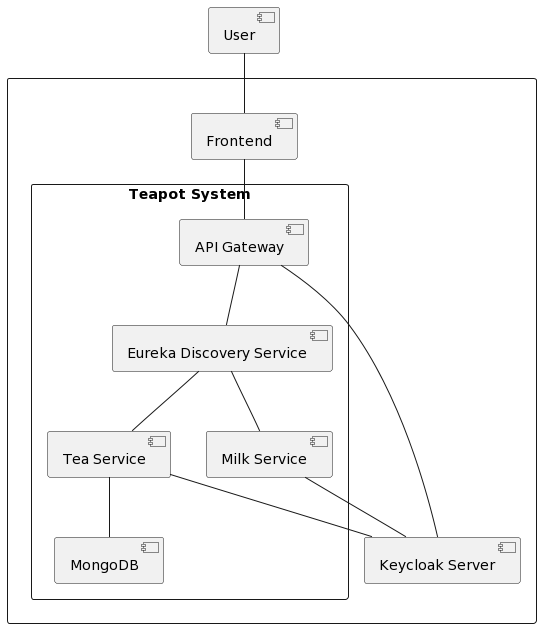
\includegraphics[height=8cm]{images/original-teapot-high-level}
	\caption{High level diagram of the implemented services and their relation to each other}
	\label{fig:original-teapot-architecture}
\end{figure}


However, since there is a lot of functionality present that is not necessary for this research, the whole system was rebuilt in a even simpler version: All that we need is the gateway and one additional service for the gateway to communicate with, and of course the keycloak server. So the Milk Service as well as the Discovery Service disappeared completely. The database still exists in the new system, but since it became clear that it would only add unnecessary overhead to the requests it is not in use anymore. Neither is the whole create/read/update/delete (CRUD) functionality. Instead, the Gateway and the Tea Service offer "hello"-endpoints that were used in the beginning for debugging. In the end, these endpoints were used for load testing, as will be described in more detail in section ???. They return a simple string message and do not require the database. This means that the gateway has two relevant endpoints: \texttt{/helloauth}, which the gateway itself responds to immediately, and  \texttt{/hellotea/name}, which is routed from the gateway to the Tea Service. \texttt{name} can be any string and will be returned in the responding message.
The remaining, stripped-down system is represented by figure \ref{fig:teapot-architecture}.
\begin{figure}[htbp]
	\centering
		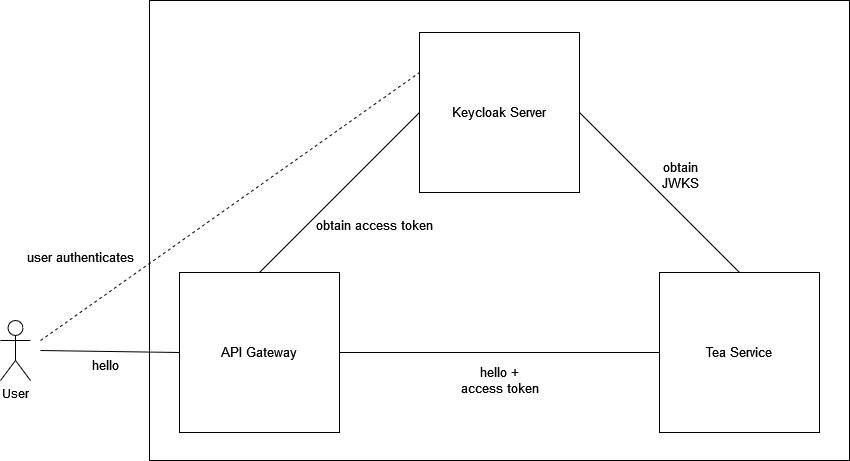
\includegraphics[height=8cm]{images/teapot-high-level}
	\caption{High level diagram of the implemented services and their relation to each other}
	\label{fig:teapot-architecture}
\end{figure}

In total, there are three versions of this system: the first version where the Gateway acts as the OAuth2 client and the Tea Service serves as the resource server, the second version where both the Gateway and the Tea Service function as resource servers, and a third version with no security implementation at all. The second version would require the inclusion of a frontend application to incorporate OAuth2 client functionality.

With this implementation, the first request to a protected resource, when the gateway hasn't obtained an access token yet, can be depicted as in figure \ref{fig:oauth2-flow-seqd}

\begin{figure}[htbp]
	\centering
		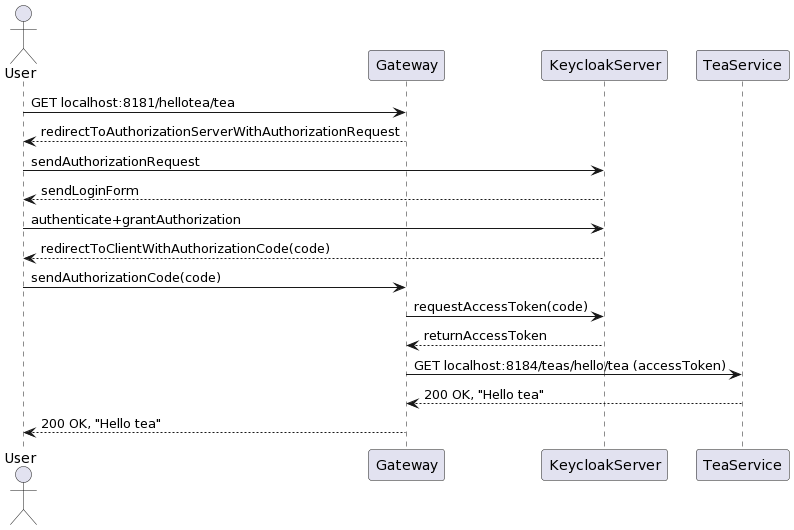
\includegraphics[height=12cm]{images/oauth2-flow_sequence-diagram}
	\caption{Sequence diagram of the first request to a protected resource including a simplified auth code grant flow}
	\label{fig:oauth2-flow-seqd}
\end{figure}

The detailed auth code grant flow has already been shown and explained in section ???, therefore a simplified version is depicted in this diagram.

Any subsequent request, as long as the access token is valid, is much simpler. The gateway already has an access token and all it has to do is append this access token to the routed request as authorization header and forward it to the Tea Service. This scenario is also used for load testing, as will be explained in section ???.

The second version does not implement a client at all. It is simply two resource servers in series. The gateway recieves an access token with the request from the user, in theory via some frontend client, in the case it is sent by a jmeter script  validates and forwards it to the Tea Service, which again validates the access token 
In both versions, the Tea Service, or the Tea Service and the Gateway respectively must obtain the JSON Web Key Set (JWKS) from the Keycloak Server, so that they will be able to validate the access token. This happens at the first request.
% detaillierte abbildungen sind hier evt. redundant... später weitermachen!

The third version is again a copy of the other two but the Keycloak Server is not needed in this case and the services do not care about authorization at all.

\section{Setup with Spring Boot and Keycloak}
\label{sec:setup-spring-boot}

\subsection{Spring and Spring Boot}

All Services in this project were developed using Spring Boot\footnote{https://spring.io/projects/spring-boot} Version 3.0. 
Spring Boot is created on top of the Spring framework, a widely used open source application framework for Java. Spring provides dependency injection and different modules, like Spring Security, Spring Test or Spring ORM (object-relational mapping), among others \cite{IntroductionSpringFramework}. Spring Boot was created in order to simplify the development of Spring-based applications by offering autoconfiguration and starter dependencies that bundle selections of libraries in one Maven or Gradle dependency \cite[pp.~4f]{wallsSpringBootAction2016}. This helps to reduce the need for the developer to write boilerplate code manually, which means that one big advantage when using Spring boot is the quick project setup. However, these configurations can be overridden or customized when needed, like it is the case for security configurations \cite[p.~50]{wallsSpringBootAction2016}, either programmatilally with Java or in many cases by adding configurations to the \texttt{applications.properties} or the \texttt{applications.yml} file \cite{CoreFeatures}. For the Teapot project the \texttt{yml} variant was used whenever possible because this way configurations are easier to write and read, and therefore they are less error-prone.

Spring Boot projects can be initialized and downloaded with the Spring Initializr\footnote{https://start.spring.io/} which is also available when creating a new Project in IntelliJ. All Maven dependencies that are needed for a project can be chosen during project creation with Spring Initializr, or they can be added later to the \texttt{pom.xml} file.

\subsection{Spring Cloud Gateway as OIDC Client}
\label{sub:gateway-cl}
%Umbenennen in The Gateway?
The Gateway's job in a MSA is to route requests to services beyond. There is a special Spring Boot starter dependency, \linebreak\texttt{spring-cloud-starter-gateway}, that was used for the implementation of the Teapot project. Maven dependencies are injected in the \linebreak\texttt{pom.xml} file in the following way:

\begin{verbatim}
        	<dependency>
            <groupId>org.springframework.cloud</groupId>
            <artifactId>spring-cloud-starter-gateway</artifactId>
        </dependency>
\end{verbatim}

With the Spring Cloud Gateway implemented, a Handler Mapping checks incoming requests for matches with configured routes and if so, forwards them to the Gateway Web Handler. The request then goes through a filterchain where route-specific pre- and post-logic is applied\cite{SpringCloudGatewaya}.

Routes can be configured in the \texttt{application.properties} file or in the \linebreak\texttt{application.yml}. Figure \ref{fig:gateway-route-config} shows an example route configuration from the \texttt{application.yml} file in the reduced Teapot project where no discovery service is used. The \texttt{uri} value is given as an environment variable and will be injected via the docker compose.yml file (!!! see docker). With the Eureka discovery service in the first Teapot, the value would be \texttt{lb://} followed by the name that the Tea service application uses to register with the discovery service. This way the Gateway does not have any need to know the specific current address of the Tea Service or any other application it is routing a request to. The \texttt{Path} predicate defines the path for the endpoint at the gateway. So in this case, requests to \texttt{http://localhost:8181/hellotea/Ula} will be recognized as a match for \texttt{\${TEAS}/teas/hello/Ula}, the path that is set under \texttt{filters} with the \texttt{SetPath}. \texttt{Ula} is an example value for the \texttt{{name}} variable.

\begin{figure}[htbp]
	\centering
		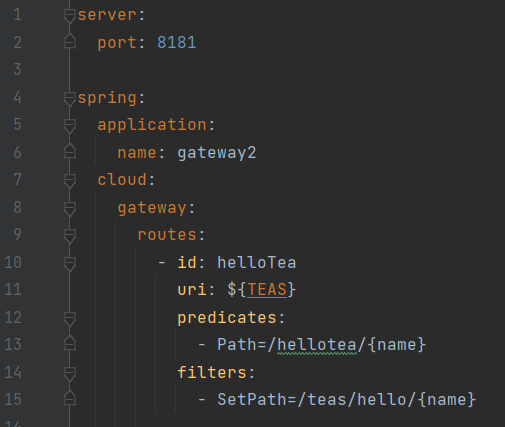
\includegraphics{images/gateway-route-config}
	\caption{Example route configuration from the Gateway's application.yml file in the reduced Teapot project}
	\label{fig:gateway-route-config}
\end{figure}

In order to configure the Gateway as OAuth2 client, we also need to include the \linebreak\texttt{spring-boot-starter-oauth2-client} dependency in the \texttt{pom.xml} file:
\begin{verbatim}
        <dependency>
            <groupId>org.springframework.boot</groupId>
            <artifactId>spring-boot-starter-oauth2-client</artifactId>
        </dependency>
\end{verbatim}

Here it is important to choose the correct starter dependency and to not get confused by the different oauth2-client dependencies available, as there are many with similar names. The \linebreak\texttt{spring-boot-starter-oauth2-client} dependency is intended to be used with Spring Boot \cite{GettingStartedSpring}. Then, after having created the client in Keycloak (see section \ref{sub:keycloak}), the application needs to be configured so it can connect to the authorization server and register with the client's credentials. All this is done in the \texttt{application.yml} file (see listing \ref{lst:clientconfig}.
\begin{lstlisting}[frame=lines, caption=OAuth2 client configuration in the Gateway's application.yml file, captionpos=b, label=lst:clientconfig, language=Java, showstringspaces=false]
spring:
[...]
  security:
    oauth2:
      client:
        provider:
          keycloak-provider:
            issuer-uri: ${keycloak.server-url}/realms/teapot
        registration:
          keycloak-gateway-client:
            provider: keycloak-provider
            scope: openid
            client-id: teapot-gateway
            client-secret: ${client-secret}
            authorization-grant-type: authorization_code
            redirect-uri: 'http://localhost:8080/login/oauth2/code/{registrationId}'
\end{lstlisting}

For this purpose we use the \linebreak\texttt{spring.security.oauth2.client.registration} base property prefix, followed by the registration id that will be used by Spring Security's \texttt{OAuth2ClientProperties} class. In this project the client's registration id is \texttt{keycloak-gateway-client}. As explained in section \ref{subsec:oidc}, \texttt{oidc} must be included in the scope claim. Further, the \texttt{client-id} and the \texttt{client-secret}, as well as the \texttt{authorization-grant-type} and the \texttt{redirect-uri} are specified. The \texttt{redirect-uri} is the address that the authorization server will send to the user agent to redirect the user back to the application after authorization has been granted (see section \ref{sec:oauth2}).
The provider section contains the provider name, in this case \texttt{keycloak-provider}. This is the name which the \texttt{registration} section refers to. The \texttt{issuer-uri} must be set correctly, otherwise the application won't be able to start successfully. This also happens when the OIDC provider is not reachable. The reason is, that the issuer-uri is used by the application to retrieve vital configuration metadata from the OIDC provider which is needed for the creation of automatic configuration. As a default, a \texttt{OpenID provider Configuration Request} is made to \texttt{"[specified issuer-uri]/.well-known/openid-configuration"}. This endpoint offers all the necessary configuration metadata, like \texttt{token\_endpoint}, \texttt{jwks\_uri}, \texttt{end\_session\_endpoint}, supported grant types and response types, supported signing and encryption algorithms etc \cite{OpenIDConnectDiscovery}.%in intro verschieben??? dann hier nur verweis

The Gateway must also be able to attach access tokens to any authorized request that will be routed to a downstream resource server. Spring Security offers a \texttt{TokenRelayGatewayFilterFactory} which fetches the access token from the authenticated user and attaches an \texttt{Authorization} header to the request with the value \texttt{"Bearer" + token}. The fastest way to add the \texttt{TokenRelayGatewayFilterFactory} is certainly to add a \texttt{default-filter} to the route configuration in the \texttt{application.yml} file as shown in listing \ref{lst:tokenrelay}. This filter will then be applied to all configured routes. Alternatively, the filter can be configured for specific routes by adding \texttt{- TokenRelay=} to \texttt{filters} \cite{TokenRelayGatewayFilterFactory}.

\begin{lstlisting}[frame=lines, caption=Route configuration with token relay default filter in the Gateway's application.yml file, captionpos=b, label = lst:tokenrelay, language=Java, showstringspaces=false]
spring:
  application:
    name: gateway2
  cloud:
    gateway:
      routes:
      
      	[...]

        - id: milk
          uri: ${MILK}
          predicates:
            - Path=/milk
          filters:
            - SetPath=/getmilk

      default-filters:
        - TokenRelay=
\end{lstlisting}

Security configuration for the gateway's endpoints can now be added in the way that is shown in the code example in listing \ref{lst:securitywebfilterchain}, taken from the reduced Teapot Gateway2. Because \texttt{/hellogateway} and \texttt{/hellotea/noauth} should remain open for testing purposes, this is taken care for with \texttt{permitAll()} before configuring all remaining endpoints as open for authenticated users only with \texttt{.authorizedExchange().anyExchange().authenticated()}. With \texttt{oauth2login()} the user will be authenticated so they can have access to the protected endpoints \cite{rozaWebClientOAuth2Support2019}. 
 
\begin{lstlisting}[frame=lines, caption=SecurityWebFilterChain for configuration of the OAuth2 client's behaviour. Code example from the reduced Teapot Gateway2, captionpos=b, label = lst:securitywebfilterchain, language=Java, showstringspaces=false]
@Configuration
@EnableWebFluxSecurity
public class Gateway2SecurityConfiguration {
    @Bean
    public SecurityWebFilterChain springSecurityWebFilterChain(
    			ServerHttpSecurity http,
    			ServerLogoutSuccessHandler handler) {
                .authorizeExchange()
                .pathMatchers("/hellogateway", "/hellotea/noauth")
                .permitAll()
            .and()
                .authorizeExchange()
                .anyExchange()
                .authenticated()
            .and()
                .oauth2Login()
            .and()
                .logout()
                .logoutSuccessHandler(handler);
        return http.build();
    }
\end{lstlisting}

%folgender absatz: ServerlogoutSuccessHander für reactive, LogoutSuccessHandler für servlet... Gateway as Client ist reactive -> ServerLogoutSuccessHandler. teas rs ist servlet, gateway as rs ist auch reactive. lohnt sich teas umschreiben auf reactive noch?
One particular aspect here is the \texttt{logoutSuccessHandler} call that gets an \texttt{ServerLogoutSuccessHandler} object as an argument. A separate bean, as shown in listing \ref{lst:logoutSuccessHandler}, has to be written in order to make this work properly. The \texttt{OidcClientInitiatedServerLogoutSuccessHandler}, which implements the ServerLogoutSuccessHandler interface, takes care of the logout process and calls the Keycloak Server's \texttt{end\_session\_endpoint} for this user \cite{AdvancedConfigurationSpring}, \cite{HowFixKeycloak2022}, \cite{rozaSpringSecurityOpenID2017}. This process is defined in OpenID Connect Session Management 1.0 as the \textit{RP-Initiated Logout}, where RP stands for relying party \cite{jonesOpenIDConnectRPInitiated2022}. Because Keycloak provides Session Management and  Discovery, the \texttt{end\_session\_endpoint} URL can be configured automatically with Spring Boot. The \texttt{postLogoutRedirectUri} is the URI that the user will be redirected to after having logged out successfully. User logout can be initiated by a \texttt{GET} or \texttt{POST} request to \texttt{{base-url}/logout} as default. The \texttt{/logout} endpoint does not need to be permitted explicitly in the filter chain \cite{rozaSpringSecurityOpenID2017}. Figures \ref{fig:logout_requests} and \ref{fig:logout_endsessionurl} show the process in the Firefox networks analytics tool. First, a POST request is sent to the Teapot Gateway's \texttt{logout} endpoint, then a redirect follows to \texttt{http://host.docker.internal:10001/realms/teapot/protocol/openid-connect/logout}, which is the \texttt{end\_session\_endpoint} at the Keycloak, together with the \texttt{id\_token\_hint} and the \texttt{post\_logout\_redirect\_uri} as query parameters. The \texttt{id\_token\_hint} is used to let Keycloak know for which user the session should be cancelled. The \texttt{post\_logout\_redirect\_uri} is open to anonymous users and doesn't require authorization.

%listing: , according to \cite{HowFixKeycloak2022} fehlt!!! einfügen hat probleme gemacht. why?
\begin{lstlisting}[frame=lines, caption=Logout success handler. Code example from the Teapot Gateway according to \cite{rozaSpringSecurityOpenID2017}, captionpos=b, label = lst:securitywebfilterchain, language=Java, showstringspaces=false]
    @Bean
    public ServerLogoutSuccessHandler keycloakLogoutSuccessHandler(ReactiveClientRegistrationRepository repository) {
        OidcClientInitiatedServerLogoutSuccessHandler oidcClientInitiatedServerLogoutSuccessHandler = new OidcClientInitiatedServerLogoutSuccessHandler(repository);
        oidcClientInitiatedServerLogoutSuccessHandler.setPostLogoutRedirectUri("https://orf.at");
        return oidcClientInitiatedServerLogoutSuccessHandler;
    }
\end{lstlisting} 

\begin{figure}[htbp]
	\centering
		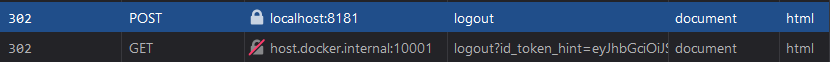
\includegraphics{images/logout_requests}
	\caption{POST request to the \texttt{\\logout} endoint of the Teapot Gateway and redirection to Keycloak's \texttt{end\_session\_endpoint}}
	\label{fig:logout_requests}
\end{figure}

\begin{figure}[htbp]
	\centering
		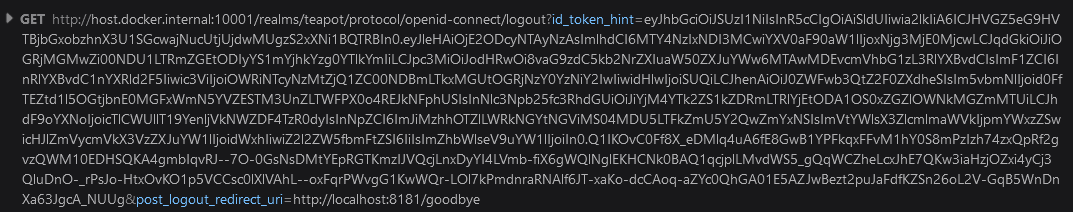
\includegraphics{images/logout_endsessionurl}
	\caption{The \texttt{end\_session\_endpoint} with query parameters}
	\label{fig:logout_endsessionurl}
\end{figure}


With Spring Boot, a \texttt{GatewayApplication.java} class is created automatically, that contains the \texttt{main} method. With this setup the Gateway application is already fully functional and able to route requests to a resource server together with an access token after the user has authenticated successfully.

An additional feature in the Teapot Gateway is the \texttt{/hellogateway} endpoint which returns a string with a greeting to the user after reading the user's name from the authentication principal . This is possible without adding an additional dependency because \texttt{Spring Cloud Gateway} already contains the \texttt{spring-boot-starter-webflux} dependency.

\begin{lstlisting}[frame=lines, caption=Reading the user's name from the authentication principal. Code Example from the Teapot Gateway., captionpos=b, label = lst:tokenrelay, language=Java, showstringspaces=false]
@RestController
public class GatewayController {
    @GetMapping("/hellogateway")
    public String greet(@AuthenticationPrincipal OAuth2User principal) {
        return "Hello, " + principal.getName() + ", from Gateway";
    }
}
\end{lstlisting}

% \texttt{spring-boot-starter-web} starter dependency also has an automatically embedded TomCat webserver (for reactive web applications there is also the \texttt{spring-boot-starter-webflux} module which comes with Netty as default). - der satz passt hier so nicht, weil gateway ja webflux hat

\subsection{The Resource Server}
\label{sub:gateway-rs}
The OAuth2 Resource Server recieves and validates the access token and, if the token is valid, grants access to the requested resource (see section \ref{sec:oauth2}). The steps to configurate a resource server with Spring Boot are not very different from the configuration of the OAuth2 client: implementation of the necessary dependencies in the \texttt{pom.xml} file, configuration of the \texttt{issure-uri}, or optionally the \texttt{jwk-set-uri} in \texttt{application.properties} or \texttt{application.properties} and overriding the default \texttt{SecurityFilterChain} with a customized one \cite{wagdeOAuthResourceServer2020}.

The minimal dependencies needed are \texttt{spring-security-oauth2-resource-server}, which contains the resource server support, and \texttt{spring-security-oauth2-jose}, which allows the resource server to decode JWTs, and is therefore crucial for the application's ability to validate JWT access tokens \cite{OAuthResourceServer}. Both are included in the \texttt{spring-boot-starter-oauth2-resource-server} starter dependency. OAuth2 bearer token authentication is possible with JWTs or with opaque tokens (see section \ref{???}). The Teapot project works with JWT.

%komisch, weil es hier für einen RS viel um authentication geht. passiert das wirklich in meinem resource server? anscheinend...
The authorization process when a request for a protected resource comes in without an access token, goes like this:
\begin{itemize}
\item An unauthenticated request comes in from the User
\item The \texttt{AuthorizationFilter} throws an \texttt{AccessDeniedException}
\item The \texttt{ExceptionTranslationFilter} initiates \textit{Start Authentication} and activates the
\texttt{BearerTokenAuthenticationEntryPoint} to send a \texttt{WWW-Authenticate: Bearer} header (see figure \ref{fig:www-authenticate}
\item The client now can retry the request with the bearer token.
\end{itemize}

\begin{figure}[htbp]
	\centering
		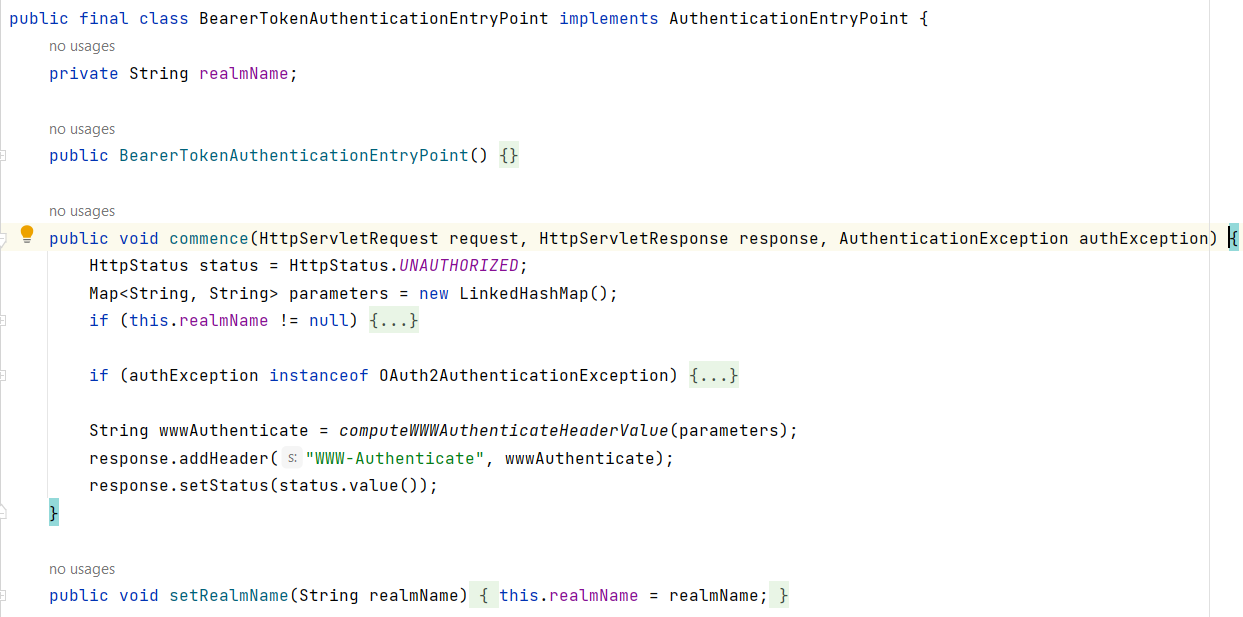
\includegraphics{images/bearertokenauthenticationenttrypoint}
	\caption{The BearerTokenAuthenticationEntryPoint sends a \texttt{WWW-Authenticate : Bearer} back to the requesting client \cite{BearerTokenAuthenticationEntryPointJava2023}}
	\label{fig:bearertokenauthenticationenttrypoint}
\end{figure}

\begin{figure}[htbp]
	\centering
		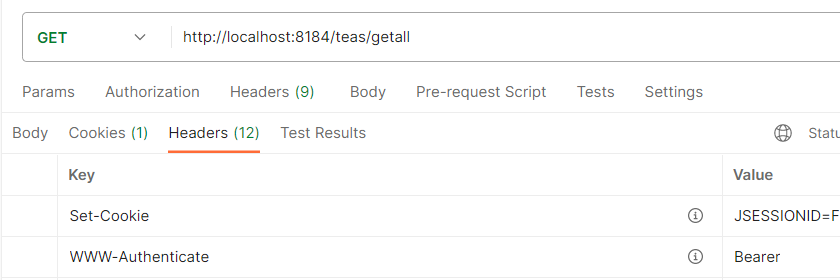
\includegraphics{images/www-authenticate}
	\caption{\texttt{WWW-Authenticate} header in the response to an unauthorized request to the resource server}
	\label{fig:www-authenticate}
\end{figure}

When the request comes with a bearer token, the \texttt{BearerTokenAuthenticationFilter} extracts the token from the \texttt{HttpServletRequest} and creates a \texttt{BearerTokenAuthenticationToken}, which implements the \texttt{Authentication} interface, represents the authenticated user and contains a \texttt{pricipal} and \texttt{authority}. An \texttt{authority} is an instance of \texttt{GrantedAuthority} and usually represents coarse-grained permission, for example \texttt{role} or \texttt{scope} \cite{ServletAuthenticationArchitecture} (see section \ref{sub:rbac}.


%!!! which is then passed to the \texttt{AuthenticationManager}. The \texttt{AuthenticationManager} is selected by the \texttt{AuthenticationManagerResolver} based on the \texttt{HttpServletRequest}, either for JWT or for opaque tokens. The \texttt{AuthenticationManager} authenticates the \texttt{BearerTokenAuthenticationToken}. Depending on wheather authentication fails or is successfull, the \texttt{SecurityContextHolder} is cleared out or set with the Authentication object. In the case of authentication failure, the \texttt{AuthenticationEntryPoint} will send the \texttt{WWW-Authenticate} header again, in the case of success, the \texttt{FilterChain} continues 

Like with the OAuth2 client, the resource server needs the \texttt{issuer-uri} to be configured correctly. At startup the resource server application has to deduce the authorization server's configuration endpoint. With only the \texttt{issuer-uri} given, it is important that one of a set of specific configuration endpoints is supported. With the Keycloak server, the configuration endpoint is \texttt{http://localhost:10001/realms/teapot/.well-known/openid-configuration}. This endpoint can now be queried for the \texttt{jwks-url} property and for supported algorithms. With this information, the application can configure the validation strategy which will in the next step query the \texttt{jwks-url} for the public key set of these algorithms. Lastly, the validation strategy will be configured to check the \texttt{iss} claim of recieved JWT access tokens against the given \texttt{issuer-uri}. For this reason the authorization server must be up and reachable, otherwise the resource server application will fail at startup \cite{OAuthResourceServer}.

In order to allow the application to start independently when the authorization server is not yet reachable, the \texttt{jkw-set-uri} can be configured explicitly, because it doesn't need to call the issuer-uri in order to find out the end point to retrieve the JWKS \cite{wagdeOAuthResourceServer2020}. In the Teapot project's \texttt{application.properties} file, this looks like in listing \ref{lst:rs-yml}. Still, with the \texttt{issuer-uri} provided, the \texttt{iss} claim in incoming JWTs will be validated against the given issuer \cite{OAuthResourceServer}.

When a request is sent to a protected endpoint at the resource server, it uses the public key from the authorization server to validate the signature and match it with the token. Then the \texttt{exp} and \texttt{iss} claims in the token are checked \cite{OAuthResourceServer}. For more fine-grained authorization it is possible to define scope and roles in Keycloak. In order to use them, custom claims have to be created at the resource server. %!!! QUELLE? und was passiert dann damit? Erklärung, warum die authorities nicht automatisch im jwt sind, gibts hier https://www.youtube.com/watch?v=j7SOIM_HL5g

\begin{lstlisting}[frame=lines, caption=\texttt{issuer-uri} and \texttt{jwk-set-uri} in the Tea service's application.properties file, captionpos=b, label = lst:rs-yml, language=Java, showstringspaces=false]
spring.security.oauth2.resourceserver.jwt.issuer-uri=${KEYCLOAK}/realms/teapot
spring.security.oauth2.resourceserver.jwt.jwk-set-uri=${KEYCLOAK}/realms/teapot/protocol/openid-connect/certs
\end{lstlisting}
%!!! für mehr platz und konsistenz: umschreiben auf yaml!

[...]

A minimal configuration of the \texttt{SecurityFilterChain} can look like in listing \ref{lst:rs-secfilterchain}. the two endpoints \texttt{/teas/hello/noauth} and \texttt{/teas/create} are open for convenience during experimental development, while all other endpoints are protected and can only be accessed with a valid access token. \texttt{oauth2ResourceServer}  takes a \texttt{Customizer} parameter of type \texttt{OAuth2ResourceServerConfigurer}. With this customizer it is possible to specify that JWT bearer tokens should be supported. This will populate the \texttt{BearerTokenAuthenticationFilter}  \cite{OAuth2ResourceServerConfigurerSpringsecuritydocsAPI}.

\begin{lstlisting}[frame=lines, caption=\texttt{SecurityFilterChain} configuration in the Tea service (resource server), captionpos=b, label = lst:rs-secfilterchain, language=Java, showstringspaces=false]
@Configuration
public class TeaSecurityConfiguration {
    @Bean
    public SecurityFilterChain filterChain(HttpSecurity http) throws Exception {
        http
                .authorizeHttpRequests().requestMatchers("/teas/hello/noauth", "/teas/create").permitAll()
                .anyRequest().authenticated();
        http.oauth2ResourceServer(OAuth2ResourceServerConfigurer::jwt);
        [...]
        return http.build();
    }
}
\end{lstlisting}

For the definition of authorities that are not provided in the original access token, the customized conversion from the JWT to an \texttt{Authentication} object can be supplied at this point as \texttt{ OAuth2ResourceServerConfigurer.JwtConfigurer.jwtAuthenticationConverter(Converter)} instead of \texttt{OAuth2ResourceServerConfigurer::jwt} \cite{OAuth2ResourceServerConfigurerSpringsecuritydocsAPI}.

Spring Security has CSRF protection enabled by default \cite{SpringBootReferencea}. Because the resource server relies on bearer token authentication, some authors in grey literature recommend making the session stateless  \cite{sandeepaUsingKeycloakSpring2023} and as a consequence to disable CSRF protection \cite{SpringaddonsSamplesTutorials}. This is only possible for resource servers, while clients that are consumed by browsers must always enable CSRF protection because they rely on session cookies \cite{lodderstedtOAuthSecurityBest2023}. This can be configured in the \texttt{SecurityFilterChain} bean as shown in listing \ref{lst:rs-stateless-csrf}.

\begin{lstlisting}[frame=lines, caption=Stateless session and disabled CSRF protection configured in the\texttt{SecurityFilterChain} bean in the Tea service (resource server), captionpos=b, label = lst:rs-stateless-csrf, language=Java, showstringspaces=false]
    @Bean
    public SecurityFilterChain filterChain(HttpSecurity http) throws Exception {
        [...]
        http.sessionManagement((session) -> session.sessionCreationPolicy(SessionCreationPolicy.STATELESS))
                .csrf().disable();
        return http.build();
    }
\end{lstlisting}


!!! Hier weiter!
was spring security damit macht:
https://docs.spring.io/spring-security/reference/servlet/oauth2/resource-server/index.html

web - starter, nicht webflux (wegen gateway?) d.h. ein servlet und eine reactive?
Ganz kurz zu DB



%Zuerst Teaservice als RS und dann nur anmerken, dass es auch das Gateway als RS gibt?



\subsection{Keycloak Server}
\label{sub:keycloak}
Was ist das
docker admin console
realms
clients
users
wie hab ich ihn configuriert?
Docker compose -> config importiert




\subsection{Role-based Access Control (RBAC) with Keycloak and Spring Boot Resource Server}
\label{sub:rbac}
%Was ist RBAC kurz allgemein mit quelle (evt. das aus BA1)

With Keycloak there is the option to define realm roles and/or client roles, which can be associated to each other to composite roles. % Quelle!!!
Figure \ref{fig:keycloak-client-roles} shows the defined client roles for the Teapot Gateway, while figure \ref{fig:keycloak-realm-roles-admin} shows one of the composite realm roles, \texttt{tea\_admin} and it's associated client role, \texttt{admin}, which belongs to the \texttt{teapot-gateway} client.

\begin{figure}[htbp]
	\centering
		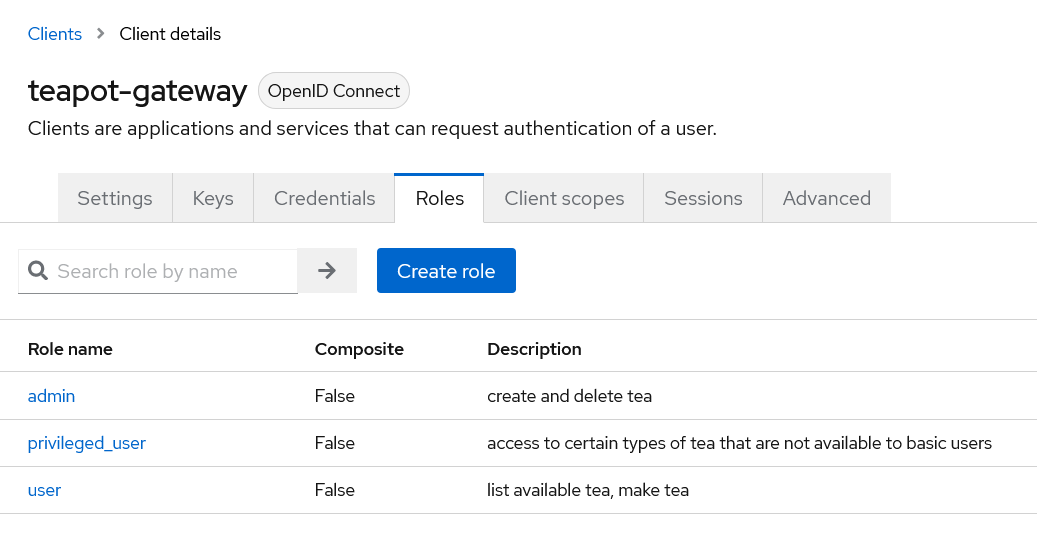
\includegraphics{images/keycloak-client-roles}
	\caption{Example of client roles defined in the Keycloak admin console}
	\label{fig:keycloak-client-roles}
\end{figure}

\begin{figure}[htbp]
	\centering
		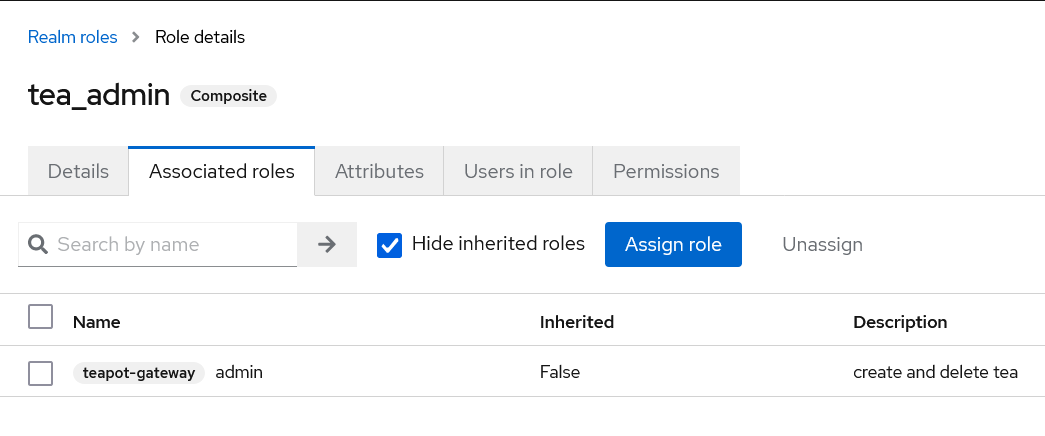
\includegraphics{images/keycloak-realm-roles-admin}
	\caption{Example of a composite realm role and it's associated client role in the Keycloak admin console}
	\label{fig:keycloak-client-roles}
\end{figure}

Keycloak includes these roles in a \texttt{realm\_access} or \texttt{resource\_access} claim respectively. The access token for a user with the \texttt{tea\_admin} realm role and the \texttt{admin} client role is shown in figure \ref{fig:keycloak-access-token}.

\begin{figure}[htbp]
	\centering
		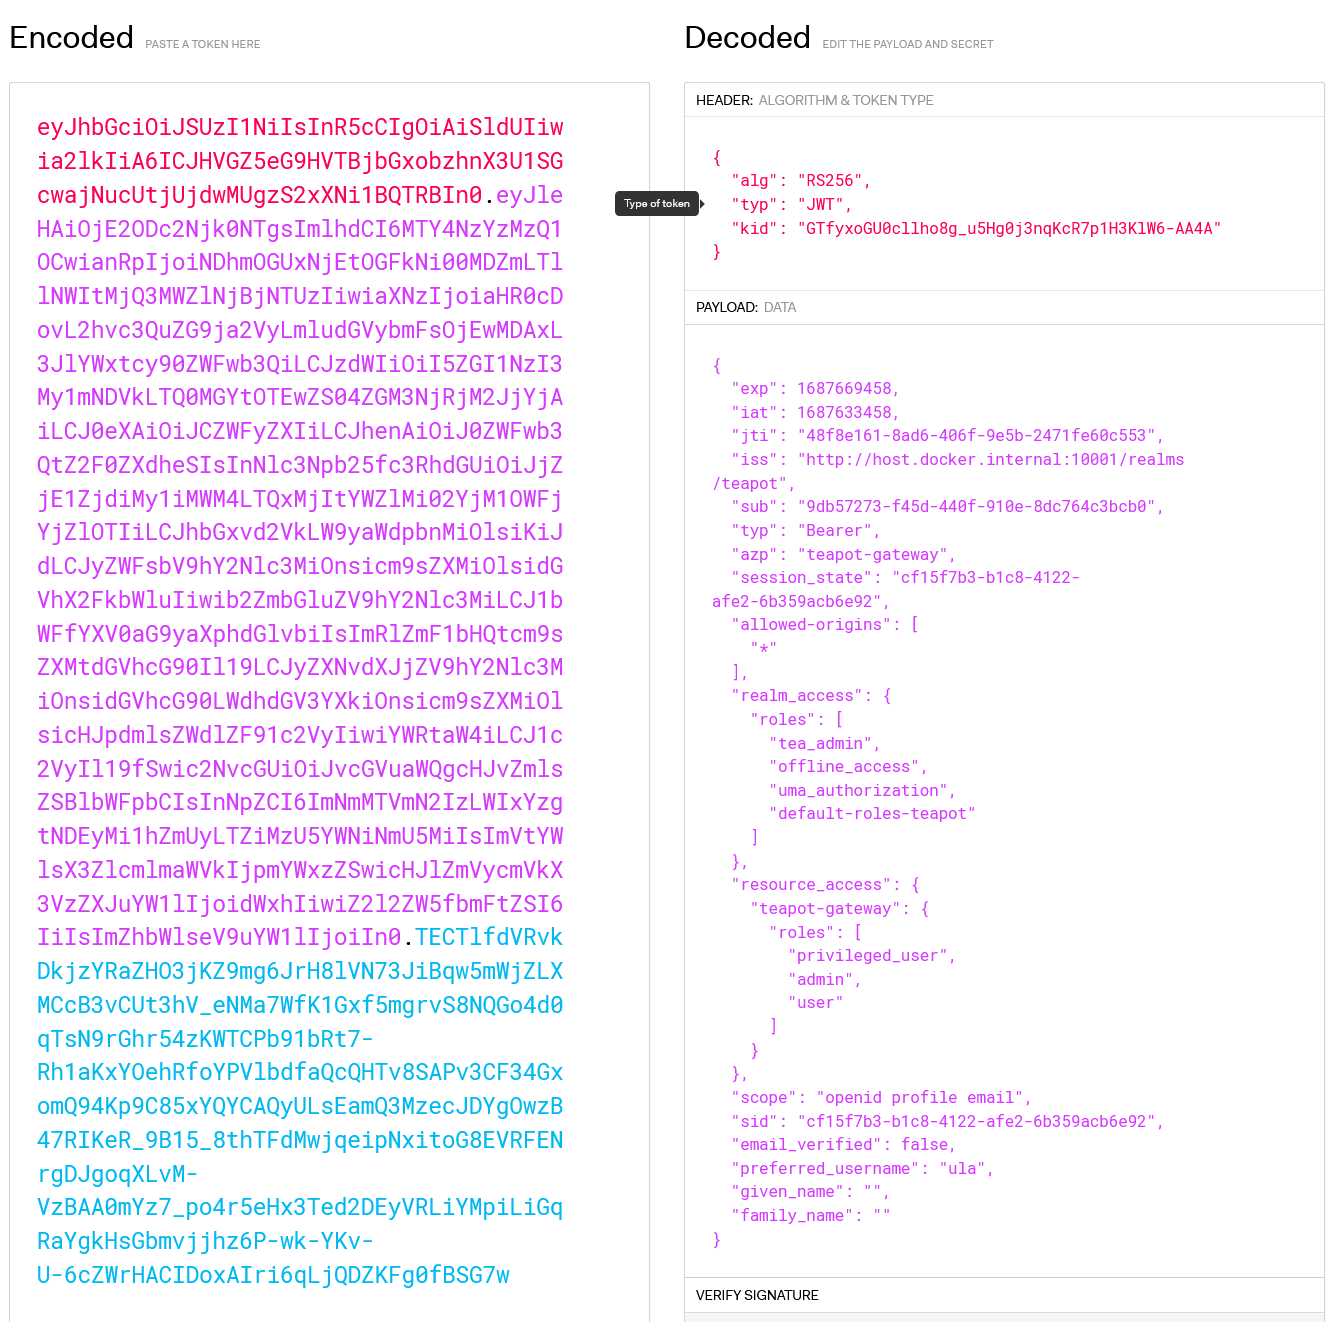
\includegraphics{images/keycloak-access-token}
	\caption{Example of an access token with claims for realm and client roles, issued by the Keycloak server}
	\label{fig:keycloak-access-token}
\end{figure}

As we can see, the access token does not contain \texttt{authority} claims. The \texttt{realm\_access} or \texttt{resource\_access} access claims are specific to Keycloak (!!! Quelle) \texttt{authority}. Spring Security allows to check for \texttt{authority} objects inside the \texttt{authentication}, but it provides no means by default to check specifically for the access claims inside a Keycloak access token. This means that these roles have no effect unless an authorities converter is added, that can translate specific claims in the access token to an \texttt{authority} in order to distinguish roles in authorization. Listing \ref{fig:rbac-authorities-converter} shows how the roles can be extracted from the specific claims in the access token. They are returned as a list of authorities and can be checked in the \texttt{SecurityFilterChain} by calling the \texttt{hasAuthority()} method. Spring Security also offers the \texttt{hasRole()} method, which checks for roles specifically. Roles are defined by the \texttt{ROLE\_} prefix. This prefix has to be added in the conversion process as well, as shown in listing \ref{fig:rbac-authorities-converter}, line 20.

\begin{lstlisting}[frame=lines, caption=Extraction of client roles and realm roles from Keycloak access token and conversion to authorities, according to \cite{ch4mpAnswerUseKeycloak2022}, simplified, with addition of the \texttt{ROLE\_} prefix., captionpos=b, label=lst:rbac-authorities-converter, language=Java]
@RequiredArgsConstructor
class JwtGrantedAuthoritiesConverter implements Converter<Jwt, Collection<? extends GrantedAuthority>> {

    @Override
    @SuppressWarnings({"rawtypes", "unchecked"})
    public Collection<? extends GrantedAuthority> convert(Jwt jwt) {
        return Stream.of("$.realm_access.roles", "$.resource_access.*.roles").flatMap(claimPaths -> {
                    Object claim;
                    try {
                        claim = JsonPath.read(jwt.getClaims(), claimPaths);
                    } catch (PathNotFoundException e) {
                        return Stream.empty();
                    }
                    final var firstItem = ((Collection) claim).iterator().next();
                    if (Collection.class.isAssignableFrom(firstItem.getClass())) {
                        return (Stream<String>) ((Collection) claim).stream().flatMap(item -> ((Collection) item).stream()).map(String.class::cast);
                    }
                    return Stream.empty();
                })
                .map(authority -> new SimpleGrantedAuthority("ROLE_" + authority))
                .map(GrantedAuthority.class::cast).toList();
    }
}\end{lstlisting}

\begin{lstlisting}[frame=lines, caption=, captionpos=b, label= lst:rbac-converter, language=Java, showstringspaces=false]
@Component
@RequiredArgsConstructor
class SpringAddonsJwtAuthenticationConverter implements Converter<Jwt, JwtAuthenticationToken> {

    @Override
    public JwtAuthenticationToken convert(Jwt jwt) {
        final var authorities = new JwtGrantedAuthoritiesConverter().convert(jwt);
        final String username = JsonPath.read(jwt.getClaims(), "preferred_username");
        return new JwtAuthenticationToken(jwt, authorities, username);
    }
}
\end{lstlisting}

!!!referenz!
\begin{lstlisting}[frame=lines, caption=, captionpos=b, label = lst:rbac-secfilterchain, language=Java, showstringspaces=false]
@Configuration
@EnableWebSecurity
public class TeaSecurityConfiguration {
    public static final String ADMIN = "tea_admin";
    public static final String USER = "user";
    public static final String PRIVILEGED_USER = "puser";

    @Bean
    public SecurityFilterChain filterChain(HttpSecurity http, Converter<Jwt, ? extends AbstractAuthenticationToken> jwtAuthenticationConverter) throws Exception {
        http
                .authorizeHttpRequests().requestMatchers("/teas/hello/noauth")
                .permitAll()
                .requestMatchers("/teas/admin", "/teas/create", "/teas/delete/**")
                .hasAuthority(ADMIN)
                .requestMatchers("/teas/maketea/special")
                .hasAnyAuthority(PRIVILEGED_USER, ADMIN)
                .requestMatchers("/teas/getall", "/teas/maketea/*", "/teas/hello/user")
                .hasAnyAuthority(USER, ADMIN, PRIVILEGED_USER)
            .anyRequest().authenticated();
        http.oauth2ResourceServer(oauth2 -> oauth2.jwt(jwt -> jwt.jwtAuthenticationConverter(jwtAuthenticationConverter)));
        http.sessionManagement((session) -> session.sessionCreationPolicy(SessionCreationPolicy.STATELESS))
                .csrf().disable();
        return http.build();
    }
}
\end{lstlisting}


\subsection{Load testing with JMeter}
\label{sub:loadtesting-jmeter}

\chapter{Results and Discussion}
\label{chap:results}

\section{Response times}
JMeter Results

\section{Code Analysis}
LoC
-> Dependencies?
+ Sonarqube Ergebnisse?

\chapter{Conclusion and Future Work}
\label{chap:conclusion}

%Keycloak adapter deprecated in 2022 https://github.com/keycloak/keycloak/discussions/10187

% additional security measurements according to https://datatracker.ietf.org/doc/html/draft-ietf-oauth-security-topics#name-access-token-leakage-at-the
\newpage
% --- Bibliography ------------------------------------------------------

%IEEE Citation [1]
\bibliographystyle{IEEEtran}
%for alphanumeric citation eg.: [ABC19]
%\bibliographystyle{alpha}

% List references I definitely want in the bibliography,
% regardless of whether or not I cite them in the thesis.

\newpage
\addcontentsline{toc}{chapter}{Bibliography}
\bibliography{BA2}

\newpage

% --- List of Figures ----------------------------------------------------

\addcontentsline{toc}{chapter}{List of Figures}
\listoffigures


% --- List of Tables -----------------------------------------------------

\newpage
\addcontentsline{toc}{chapter}{List of Tables}
\listoftables

\end{document}
